\subsection{Fórum}
O desenvolvimento da página de fórum trouxe diversas dificuldades entre elas a gestão de filtros, pesquisas, a mostragem de publicações e atualização das mesmas.


\vspace{10mm}
\begin{figure}[htb]%
  \centering
  \subfloat[\centering Página de forum]{{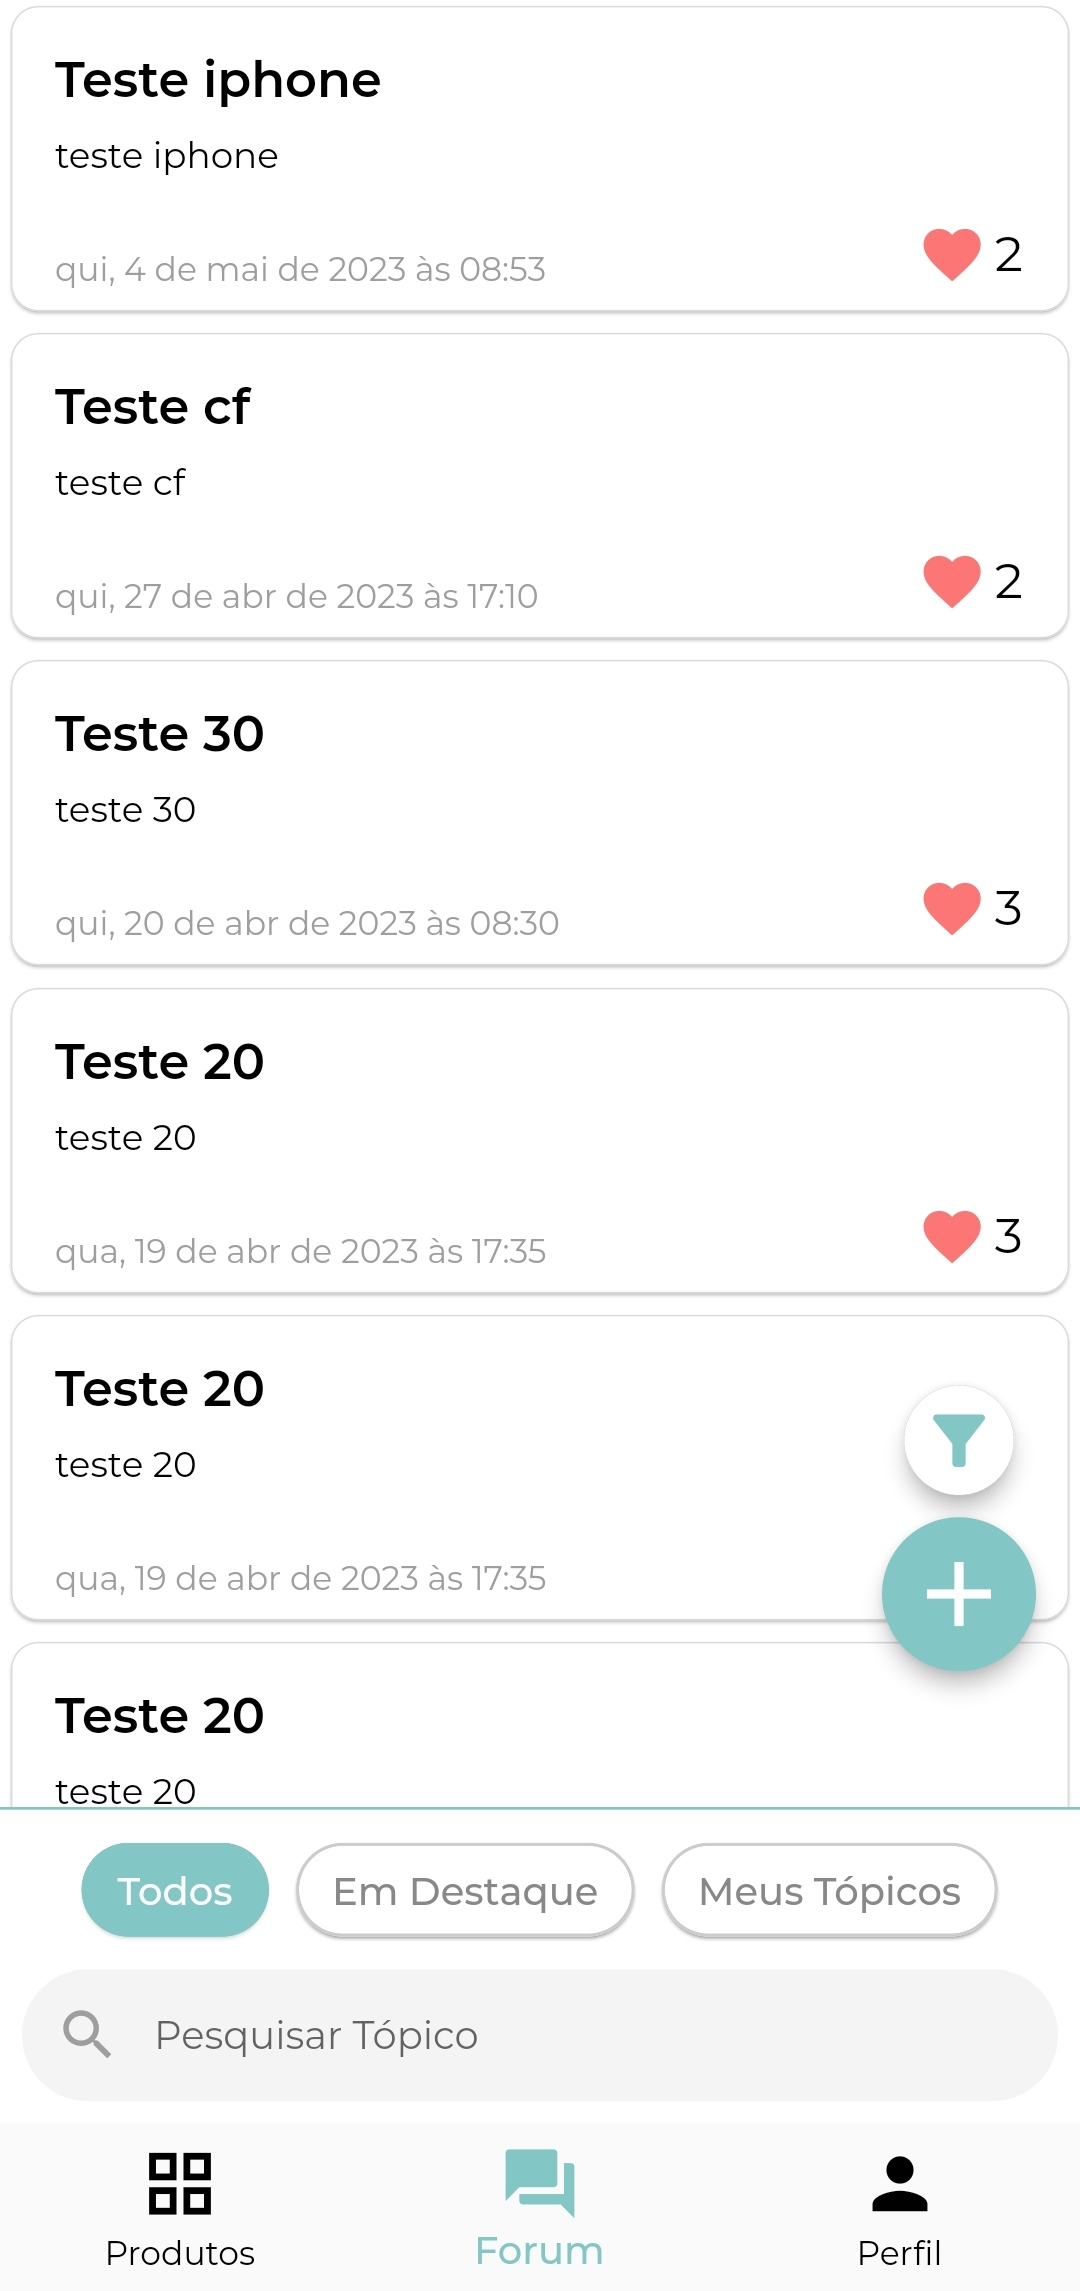
\includegraphics[width=0.3\textwidth]{images/implementacao/frontend/forum/1686055611203.jpg} }}%
  \qquad
  \subfloat[\centering Filtragem de tipo]{{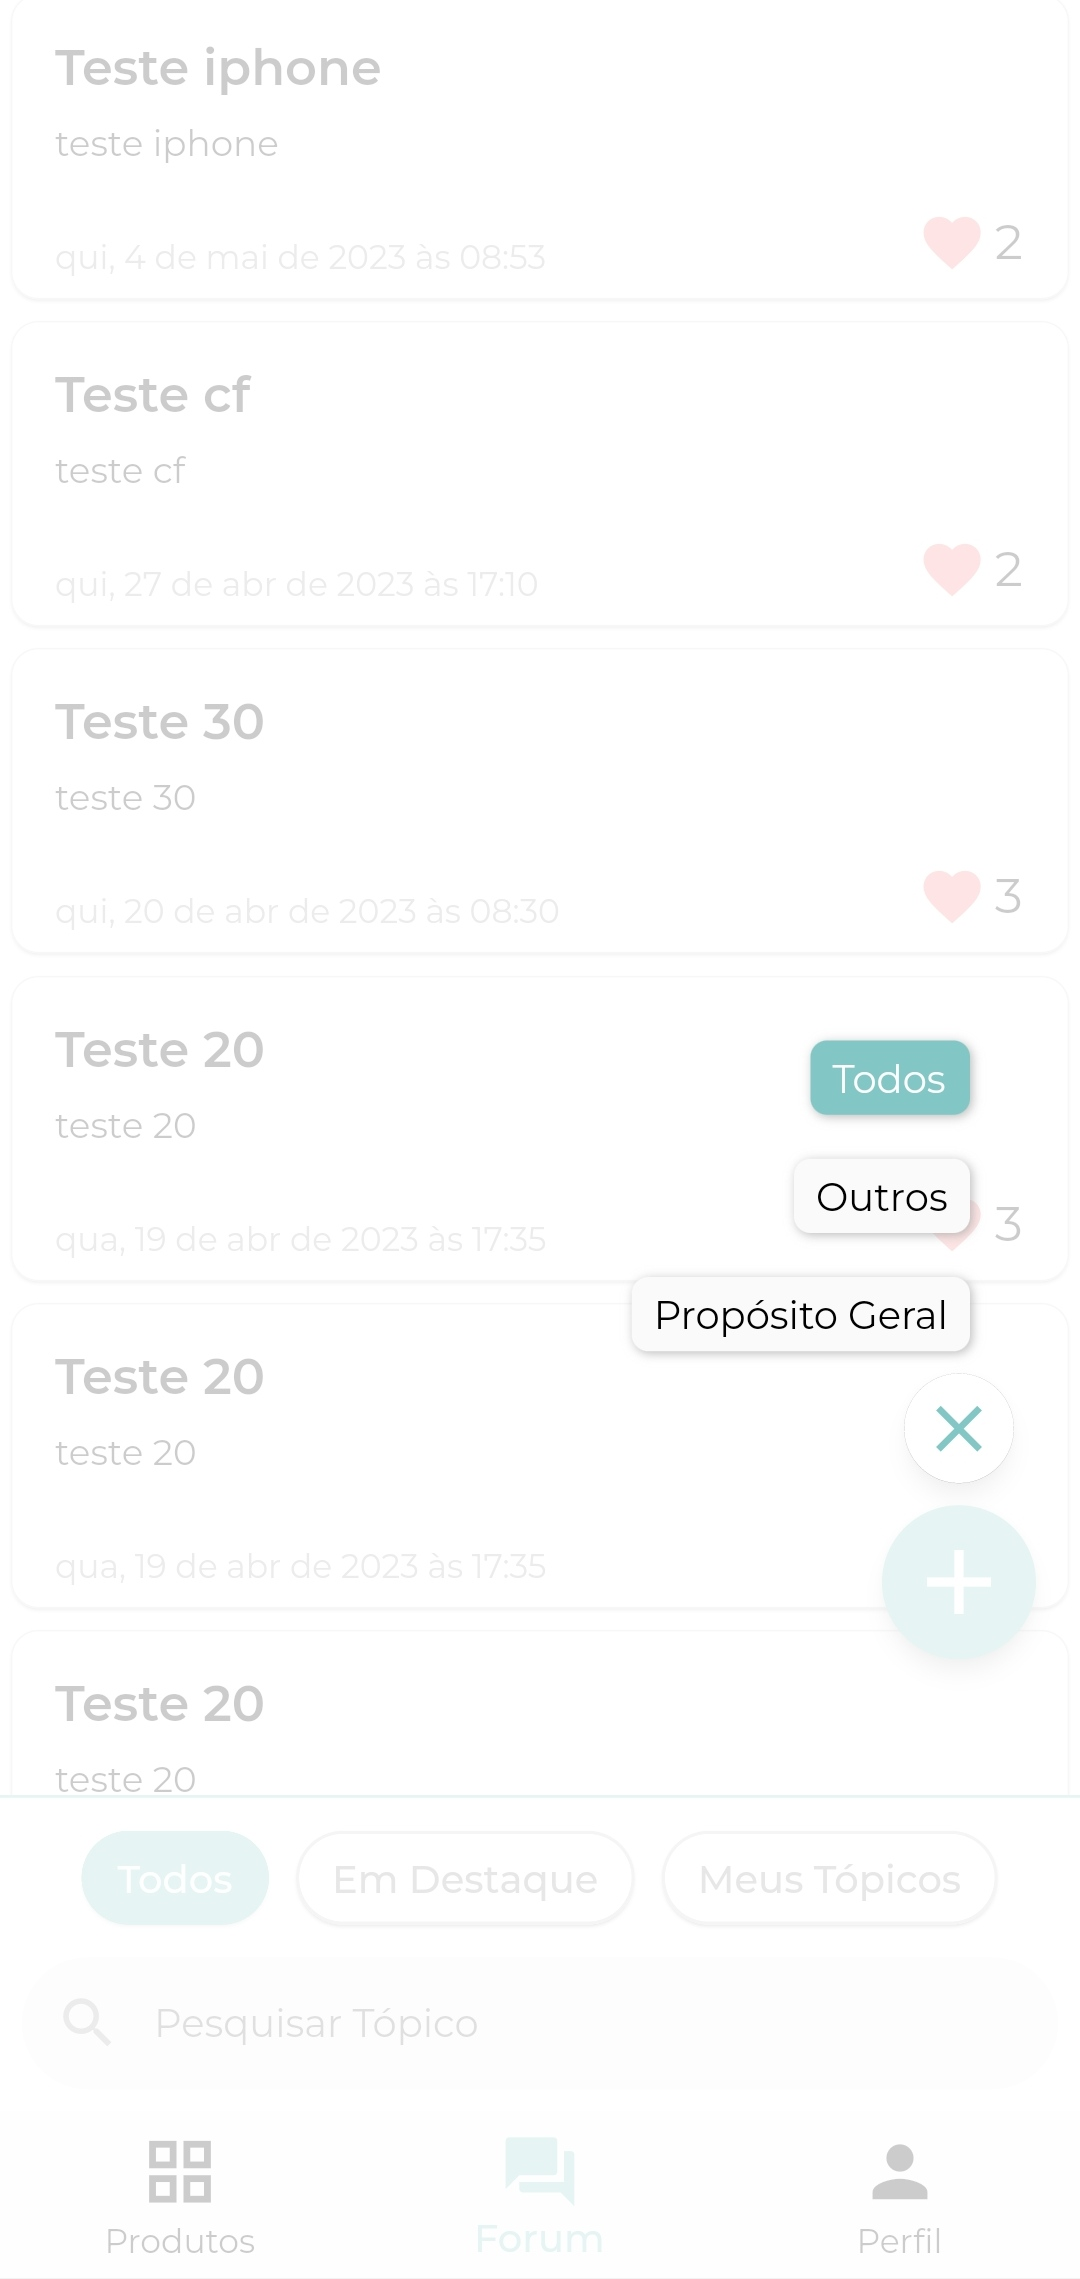
\includegraphics[width=0.3\textwidth]{images/implementacao/frontend/forum/1686055611213.jpg} }}%
  \label{fig:72}%
\end{figure}
\vspace{10mm}

\newpage

\subsubsection{Filtragem de tópicos}
O grande problema com a filtragem dos tópicos é que existem 3 tipos de filtros, o de categoria de tópico, o de tipo de tópico e o de pesquisa. 

Uma vez que algum filtro seja alterado, os seguintes deverão ser novamente executados para garantir que todos se encontram aplicados. Inicialmente este tipo de filtragem não era executado, o que levava a problemas, como por exemplo, sempre que se efetua uma pesquisa, esta não era efetuada sobre as publicações filtradas o que levava a que a pesquisa fosse efetuada por todas as publicações.

Outro problema encontrado foi a troca de categoria, por vezes acontecia que os filtros de categoria adicionavam-se o que levava a que estes não mostrassem publicações.

Sendo assim foram criados métodos para auxílio na filtragem, assim como uma prioridade, sendo que a cada método invoca o método seguinte de forma encadeada. Primeiramente aplica-se o filtro de categoria, de seguida este envia o resultado para o método de filtragem por tipo e por fim se existir algum tipo de pesquisa os tópicos serão filtrados pela mesma.

\begin{figure}[htb]
  \centering
  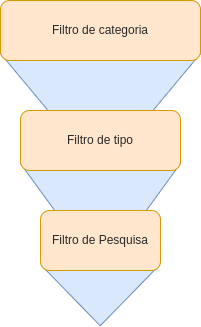
\includegraphics[width=0.25\textwidth]{images/implementacao/frontend/forum/filtros/filtros.png}
  \caption{Filtragem do forum}
  \label{fig:73}
\end{figure}

\newpage

\subsubsection{Carregamento de tópicos}
Inicialmente o carregamento de tópicos fazia-se por inteiro, desde carregamento de todos os tópicos, até todos os dados dos mesmos, pois visto que não existiam muitos tópicos este não seria um problema para a \textit{API}, mas conforme os testes foram realizados, a quantidade de tópicos existentes foi aumentando, pelo que foi possível visualizar o tempo de demora de resposta do servidor a aumentar, assim como também o desempenho da aplicação no fórum a piorar.

A resolução deste problema provei com com uma técnica de sliding window, na qual os tópicos se mantêm carregados, sendo que a própria \textit{framework} consegue através da lista retirar de renderização os tópicos que o utilizador não consegue ver. 

Esta solução foi implementada através da utilização de 3 valores, quantidade de tópicos a obter, índice inicial e data do primeiro tópico. O valor de quantidade de tópicos a obter, inicialmente 10, permite limitar a quantidade de tópicos que a API irá processar o que reduz o tempo de resposta. O índice inicial, permite indicar qual o índice do primeiro elemento que se deseja obter da lista. A data do primeiro tópico, permite manter uma referência temporal para obter tópicos, o que garante que a lista que se está a visualizar é sempre a mesma.

\begin{figure}[htb]
  \centering
  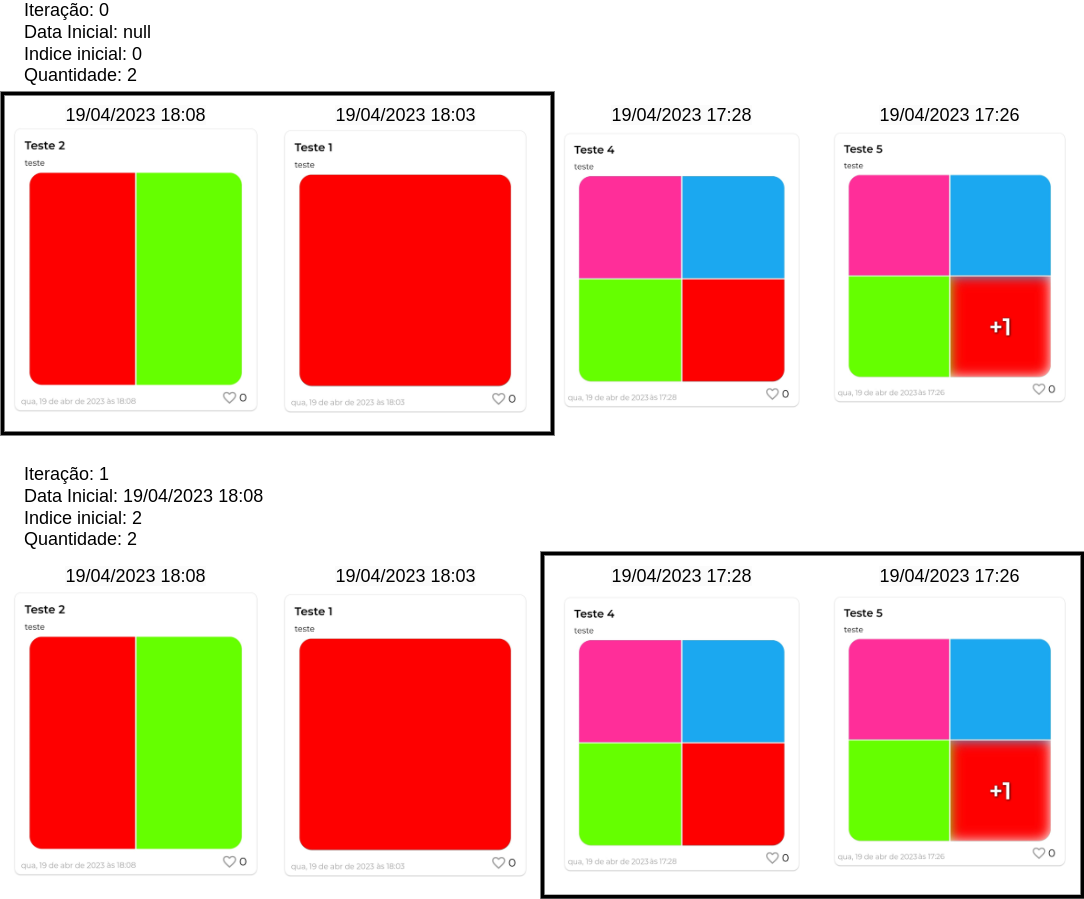
\includegraphics[width=0.8\textwidth]{images/implementacao/frontend/forum/loading_topics/topics_loading.png}
  \caption{Carregamento de tópicos}
  \label{fig:74}
\end{figure}

Foi também reduzida a quantidade de dados carregados por cada tópico, pelo que apenas os comentários diretos à publicação são carregados e não as respostas a estes, o que também contribuiu para a melhoria de desempenho.

Por fim sempre que o utilizador alcança o fim da lista de tópicos este poderá deslizar para carregar mais tópicos.

\newpage

\subsubsection{Detalhes de tópico}

A página de detalhes de tópico sofreu os mesmos problemas que a página anterior pelo que foi necessário aplicar a mesma solução sobre os comentários de tópico e sobre as respostas aos mesmos. Sendo assim são carregados os primeiros 10 comentários e por fim mostrado ao utilizador quantos mais existem que poderá carregar, sendo carregados 10 de cada vez.

Estes comentários podem também conter respostas sendo que estas podem ser carregadas também 10 de cada vez e o utilizador consegue esconder ou mostrar estas.

Outro problema que surgiu no desenvolvimento da página de detalhes de tópico foi o destaque de um comentário. Este foi um grande problema, pois com a nova implementação as mensagens não se encontram carregadas no momento de destacar a mensagem, pelo que, é necessário procurar a mesma nos comentários carregados, o que expande assim as respostas do comentário que contêm a reposta a destacar.

O destacamento de mensagens também continha um erro, onde sempre que algo no ecrã é atualizado, este recarregava a animação de destaque, pelo que este código teve de ser movido para apenas ser executado no momento de inicialização do ecrã após todos os elementos se encontrarem devidamente carregados.

\begin{figure}[htb]
  \centering
  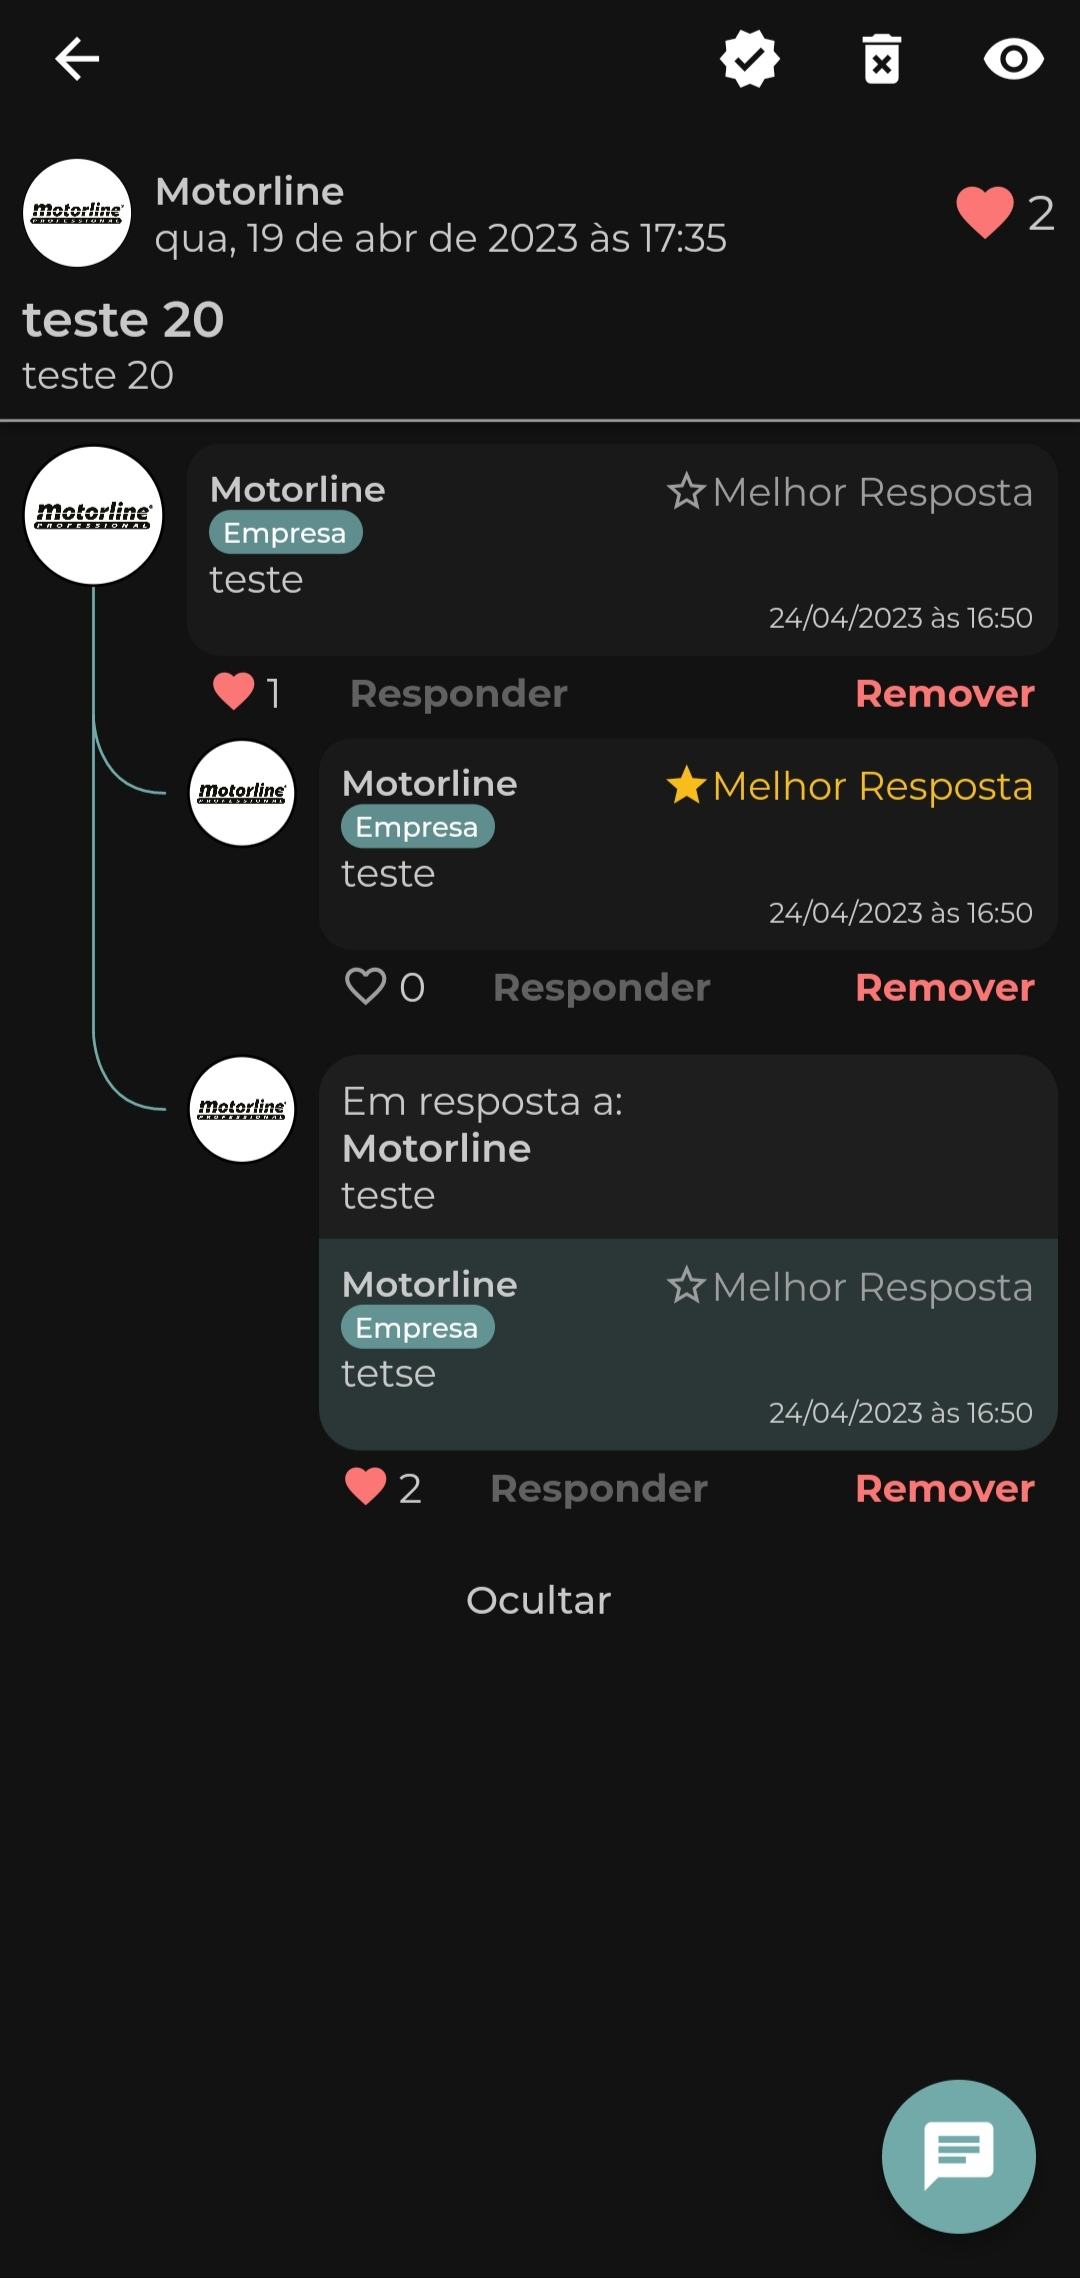
\includegraphics[width=0.35\textwidth]{images/implementacao/frontend/forum/loading_topics/1686062701127.jpg}
  \caption{Destaque de mensagens}
  \label{fig:75}
\end{figure}